\chapter{Appendix}
\label{ch:appendix}

\section{Prompts}
\label{app:prompts}

The prompt-intervention experiment changes only the generation prompt, so the prompts are reproduced below.
The prompts are reproduced exactly as used in the experiments.

The baseline arm uses~\cref{lst:prompt-gen} alone.
The idiom arm uses the base system prompt followed by the idiom guide (\cref{lst:prompt-idiom}).
The two schema-evidence arms append a per-question schema card, and \cref{lst:schema-cards} shows one card of each form; the code that builds the cards is in the accompanying repository.
Disambiguation (\cref{lst:prompt-disamb}) is identical in every arm.

\begin{lstlisting}[caption={Generation system prompt (baseline).},label={lst:prompt-gen},basicstyle=\ttfamily\scriptsize,breaklines=true,captionpos=b]
You are a SPARQL expert for Wikidata. Generate a SPARQL query that
answers the question, but instead of using opaque Wikidata IDs, use human-readable
labels in this exact bracket format:
  - For entities:   wd:[entity:LABEL]      e.g. wd:[entity:Christopher Nolan]
  - For properties: wdt:[property:LABEL]   e.g. wdt:[property:director]
Use this format for ALL entities and properties. Keep variable names and SPARQL
structure normal. Output ONLY the SPARQL query, no explanation.
\end{lstlisting}

\begin{lstlisting}[caption={Disambiguation prompt, as built by the pipeline. The candidate list is injected at \texttt{\{cand\_text\}}. The reported runs send this prompt through Anthropic's batch interface or, for the open models, through vLLM. If the answer contains no identifier, or a request fails, the first search result is used instead; in the reported frontier-model runs all 4,063 requests returned an answer line, so this fallback was never used.},label={lst:prompt-disamb},basicstyle=\ttfamily\scriptsize,breaklines=true,captionpos=b]
def disambiguate(question, label, candidates, is_property=False):
    if not candidates:
        return ""
    if len(candidates) == 1:
        return candidates[0]["id"]
    kind = "property" if is_property else "entity"
    cand_text = "\n".join(
        f"  {c['id']}: {c['label']} — {c['description'] or '(no description)'}"
        for c in candidates)
    example_id = "P57" if is_property else "Q25191"
    prompt = f"""Question: "{question}"

Find the correct Wikidata {kind} ID for: "{label}"

Candidates:
{cand_text}

Think step by step about which candidate best fits the {kind} "{label}" in the
context of the question. Output ONLY the chosen ID (e.g. {example_id}) on the last
line, prefixed with "ANSWER: ".
"""
\end{lstlisting}

\begin{lstlisting}[caption={Idiom-guidance prompt. The idiom arm is \textsc{base} followed by \textsc{idiom guide}; the baseline arm is \textsc{base} alone.},label={lst:prompt-idiom},basicstyle=\ttfamily\scriptsize,breaklines=true,captionpos=b]
You are a SPARQL expert for Wikidata. Generate a SPARQL query that
answers the question, but instead of using opaque Wikidata IDs, use human-readable
labels in this exact bracket format:
  - For entities:   wd:[entity:LABEL]      e.g. wd:[entity:Christopher Nolan]
  - For properties: wdt:[property:LABEL]   e.g. wdt:[property:director]
Use this format for ALL entities and properties. Keep variable names and SPARQL
structure normal. Output ONLY the SPARQL query, no explanation.

Before writing the query, consider which of Wikidata's modelling idioms the
question requires. Use them where appropriate:

1. Class membership is usually hierarchical. A question about a category
   normally means the category and all of its subclasses, so prefer
   ?item wdt:[property:instance of]/wdt:[property:subclass of]* wd:[entity:CLASS]
   over a direct instance-of triple. Use the direct form only when the question
   clearly means the class itself.

2. Values that carry extra information live on statements, not on direct
   claims. When the question asks about a qualifier — a date, a rank, a role, a
   plot, a part something applies to — go through the statement node:
     ?item p:[property:P] ?st .
     ?st ps:[property:P] ?value ; pq:[property:QUALIFIER] ?qvalue .
   Direct wdt: triples cannot see qualifiers.

3. Quantities with units, precision or bounds require the statement value node:
     ?item p:[property:P]/psv:[property:P] ?vn .
     ?vn wikibase:quantityAmount ?amount ; wikibase:quantityUnit ?unit .
   Use this whenever units must be compared or converted.

4. Questions about words, forms, senses or languages concern lexemes, not
   items: use wikibase:lemma, dct:language, ontolex:sense and the lexeme
   namespace rather than item properties.

5. Counting, ranking or "how many / most / per X" questions need explicit
   aggregation: COUNT/SUM with GROUP BY, and ORDER BY ... DESC for ranking.

6. Alternatives in the question ("mathematicians or physicists", several
   platforms) are expressed with VALUES or UNION, not by choosing one.

7. Do not add LIMIT unless the question asks for a specific number of results.

Apply only the idioms the question actually calls for; do not add machinery
that is not needed.
\end{lstlisting}

\begin{lstlisting}[caption={Schema-card construction: the first function produces the verbose arm's evidence and the second the targeted arm's.},label={lst:prompt-schema},basicstyle=\ttfamily\scriptsize,breaklines=true,captionpos=b]
def build_card(entities, properties, prop_cache, ent_cache):
    """Compose the compact evidence text placed in the generation prompt.
    Entity evidence is included when the question mentions entities; property
    evidence is always included, so property-only questions are covered too."""
    lines = []
    for qid in entities[:MAX_ENTS]:
        info = ent_cache.get(qid)
        if not info:
            continue
        head = f"{qid} ({info['label']})"
        if info["is_class"]:
            head += " — this is a class with subclasses; a question about it " \
                    "usually means the class and everything below it"
        lines.append(head)
        if info["properties"]:
            named = ", ".join(f"{p} ({prop_cache.get(p, {}).get('label', p)})"
                              for p in info["properties"][:MAX_PROPS])
            lines.append(f"  properties in use: {named}")
        if info["qualified"]:
            named = ", ".join(f"{p} ({prop_cache.get(p, {}).get('label', p)})"
                              for p in info["qualified"][:8])
            lines.append(f"  statements with qualifiers (need p:/pq: to read "
                         f"the qualifier): {named}")
        quants = [p for p in info["properties"]
                  if prop_cache.get(p, {}).get("quantity")]
        if quants:
            lines.append(f"  quantity-valued (unit lives on the value node, "
                         f"need p:/psv:): {', '.join(quants[:6])}")

    prop_lines = []
    for pid in properties[:MAX_PROPS]:
        info = prop_cache.get(pid)
        if not info:
            continue
        bits = []
        if info.get("qualifiers"):
            named = ", ".join(f"{q} ({prop_cache.get(q, {}).get('label', q)})"
                              for q in info["qualifiers"][:5])
            bits.append(f"used with qualifiers {named}, reachable only through "
                        f"p:/pq:")
        if info.get("quantity"):
            bits.append("quantity-valued; the unit sits on the statement value "
                        "node, reachable through p:/psv:")
        if info.get("class_range"):
            bits.append("its values are classes with subclasses, so filtering "
                        "on one usually needs P279* closure")
        if bits:
            prop_lines.append(f"{pid} ({info.get('label', pid)}): " + "; ".join(bits))
    if prop_lines:
        lines.append("properties this question refers to:")
        lines += ["  " + l for l in prop_lines]
    return "\n".join(lines)

def build_card_targeted(entities, properties, prop_cache, ent_cache):
    """Targeted variant: evidence ONLY for the properties/entities the
    question actually links to (gold mentions), no enumeration of everything
    an entity happens to carry. Tests whether the full-listing version failed
    from information overload/distraction rather than from the concept of
    grounding itself."""
    lines = []
    for qid in entities[:MAX_ENTS]:
        info = ent_cache.get(qid)
        if info and info.get("is_class"):
            lines.append(f"{qid} ({info['label']}) is a class with subclasses: "
                         f"a question about it usually means the class and "
                         f"everything below it (wdt:[property:instance of]/"
                         f"wdt:[property:subclass of]*).")
    seen = set()
    for pid in properties[:MAX_PROPS]:
        info = prop_cache.get(pid)
        if not info or pid in seen:
            continue
        seen.add(pid)
        label = info.get("label", pid)
        bits = []
        if info.get("qualifiers"):
            bits.append("if the question asks for something beyond the plain "
                        "value (e.g. a date, role or extra detail attached to "
                        "this fact), it is recorded as a QUALIFIER and needs "
                        "p:[property:" + label + "] / pq:[property:...], not "
                        "wdt:[property:" + label + "] alone")
        if info.get("quantity"):
            bits.append("its value is a QUANTITY with a unit; if the unit or "
                        "precision matters, use p:/psv: to reach the value node")
        if info.get("class_range"):
            bits.append("its value is itself a class; if the question means "
                        "the value or anything below it, add "
                        "wdt:[property:subclass of]* on the value")
        if bits:
            lines.append(f"{pid} ({label}): " + "; ".join(bits) + ".")
    return "\n".join(lines)
\end{lstlisting}

\begin{lstlisting}[caption={Example schema cards, one of each form, as supplied to the generator.},label={lst:schema-cards},basicstyle=\ttfamily\scriptsize,breaklines=true,captionpos=b]
--- verbose card (row 0) ---
properties this question refers to:
  P625 (coordinate location): used with qualifiers P2241 (reason for deprecated rank), P459 (determination method or standard), P518 (applies to part), P609 (terminus location), P813 (retrieved), reachable only through p:/pq:

--- targeted card (row 0) ---
P625 (coordinate location): if the question asks for something beyond the plain value (e.g. a date, role or extra detail attached to this fact), it is recorded as a QUALIFIER and needs p:[property:coordinate location] / pq:[property:...], not wdt:[property:coordinate location] alone.
\end{lstlisting}


\section{Full Result Tables}
\label{app:tables}

The results chapter reports the main comparisons on the common subset. The tables below provide the full results, including per-run denominators, complexity breakdowns, and confidence intervals.
The tables below provide the full results with per-run denominators, breakdowns by complexity, and complete interval estimates.

\begin{table}[htbp]
\centering
\footnotesize
\caption{Full strict-set results with per-run denominators, working split.}
\label{tab:app-master}
\resizebox{\ifdim\width>\textwidth\textwidth\else\width\fi}{!}{%
\begin{tabular}{@{}lrrrrrrr@{}}
\toprule
Approach & Questions scored & Pooled (\%) & Simple & Medium & Complex & Entity-level (\%) & Entity rows \\ \midrule
Zero-shot GPT-5.4 & 400 & 12.8 & 21.7 & 13.1 & 10.7 & 14.7 & 350 \\
Zero-shot Claude Opus 4.8 & 400 & 17.8 & 29.7 & 18.8 & 14.2 & 21.7 & 355 \\
Zero-shot Gemini 3.1 Flash Lite & 400 & 8.6 & 13.9 & 10.4 & 5.4 & 9.8 & 342 \\
Zero-shot DeepSeek V4 Flash & 400 & 10.4 & 21.2 & 11.2 & 7.4 & 12.5 & 346 \\
Few-shot GPT-5.4 & 400 & 14.9 & 33.2 & 14.9 & 11.2 & 17.1 & 355 \\
Few-shot Claude Opus 4.8 & 400 & 18.7 & 36.9 & 19.4 & 14.2 & 22.4 & 357 \\
Few-shot Gemini 3.1 Flash Lite & 400 & 10.8 & 14.1 & 12.5 & 8.1 & 13.1 & 346 \\
Few-shot DeepSeek V4 Flash & 400 & 10.3 & 24.7 & 10.5 & 7.1 & 11.7 & 348 \\
Gold-label condition & 390 & 94.9 & 97.1 & 95.8 & 93.4 & 97.1 & 317 \\
End-to-end pipeline & 400 & 22.4 & 32.3 & 25.5 & 16.8 & 27.5 & 363 \\
\bottomrule
\end{tabular}}
\tabnote{All 400 strict-set questions count in the pooled columns, and a question without a scored query counts as zero (the gold-label condition has no labelled query for ten of them). Entity-level Jaccard is averaged over the questions on which it is defined for each run; their number is given in the last column.}
\end{table}

\begin{table}[htbp]
\centering
\footnotesize
\caption{Pipeline stage outcomes on the official split.}
\label{tab:app-official}
\resizebox{\ifdim\width>\textwidth\textwidth\else\width\fi}{!}{%
\begin{tabular}{@{}lrrrr@{}}
\toprule
Metric & simple & medium & complex & overall \\ \midrule
Generated labelled query (\%) & 92.9 & 97.4 & 97.0 & 96.8 \\
Fully linked (\%) & 92.9 & 93.7 & 90.9 & 92.1 \\
Executed (\%) & 88.1 & 91.6 & 84.0 & 87.3 \\
Strict fair Jaccard (\%) & 44.3 & 26.3 & 15.0 & 23.4 \\
\bottomrule
\end{tabular}}
\tabnote{Stage rates are over all 495 questions of the split; Jaccard is over all 370 strict-set questions, and a question without a generated query counts as zero.}
\end{table}

\begin{table}[htbp]
\centering
\footnotesize
\caption{Linking F1 with bootstrap confidence intervals.}
\label{tab:app-linker-ci}
\resizebox{\ifdim\width>\textwidth\textwidth\else\width\fi}{!}{%
\begin{tabular}{@{}lrrr@{}}
\toprule
Linker or paired difference & F1 / difference & 95\% CI low & 95\% CI high \\ \midrule
Reasoning (Opus 4.8) & 97.7 & 96.8 & 98.5 \\
Reasoning (Qwen 14B) & 94.9 & 93.6 & 96.3 \\
Reasoning (Qwen 7B) & 95.8 & 94.5 & 96.9 \\
GLiNKER (bi-encoder) & 72.8 & 70.0 & 75.4 \\
ELQ (fine-tuned) & 28.4 & 25.2 & 31.7 \\
ReFinED (fine-tuned) & 26.6 & 23.2 & 29.8 \\
First search result & 93.5 & 92.1 & 95.0 \\
Reasoning (Opus 4.8) - GLiNKER (bi-encoder) & 24.9 & 22.3 & 27.7 \\
Reasoning (Qwen 14B) - GLiNKER (bi-encoder) & 22.2 & 19.4 & 25.1 \\
Reasoning (Qwen 7B) - GLiNKER (bi-encoder) & 23.0 & 20.3 & 25.8 \\
Reasoning (Opus 4.8) - First search result & 4.1 & 2.7 & 5.6 \\
Reasoning (Qwen 14B) - First search result & 1.4 & -0.4 & 3.1 \\
Reasoning (Qwen 7B) - First search result & 2.2 & 0.6 & 3.9 \\
\bottomrule
\end{tabular}}
\tabnote{$B = 2{,}000$ resamples over the 1,086 entity mentions every linker scored; the same resample is applied to all linkers on each draw.}
\end{table}


Larger tables are provided in the accompanying repository, including the complete construct-usage and agreement matrices, selector results, label-failure taxonomy, repair results, and query-log construct prevalence.

\section{Error-Analysis Annotations}
\label{app:annotations}

All thirty annotated cases from the reported end-to-end run are listed below. This allows the failure categorisation to be checked independently.
The sample is complexity-stratified with seed 42.
The questions and notes are truncated for width, and the full records, including both queries, are in the accompanying repository.

\footnotesize\sloppy
\begin{longtable}{@{}r >{\raggedright\arraybackslash}p{1.7cm} >{\raggedright\arraybackslash}p{4.6cm} >{\raggedright\arraybackslash}p{2.5cm} >{\raggedright\arraybackslash}p{4.4cm}@{}}
\caption{All thirty annotated failure cases.}\label{tab:app-annotations}\\
\toprule
ID & Complexity & Question & Category & Annotator note \\ \midrule
\endfirsthead
\multicolumn{5}{@{}l}{\footnotesize\itshape continued from previous page}\\
\toprule ID & Complexity & Question & Category & Annotator note \\ \midrule
\endhead
\midrule \multicolumn{5}{r@{}}{\footnotesize\itshape continued overleaf}\\
\endfoot
\bottomrule
\endlastfoot
32 & simple & What are the nodes and predicates related to 'Wikidata' in English? & \texttt{triple\_flip} & gold matches the literal "Wikidata"@en as OBJECT (?node ?predicate "Wikidata"@en); mine starts from wd:Q2013 as SUBJECT. Linking succeeded but the qu\ldots{} \\
8 & simple & List all literary works and their descriptions. & \texttt{execution} & result\_too\_large: mine uses wdt:P31 where gold uses wdt:P279, matching every literary work rather than its subclasses, so the result exceeds the 50MB\ldots{} \\
3 & simple & List politicians who have Mastodon accounts. & \texttt{near\_miss} & same properties P4033/\allowbreak{}P106 and same shape; gold additionally joins P27 country and projects countryLabel, mine omits it \\
14 & simple & List the top 20 humans with the highest recorded weight. & \texttt{benchmark\_noise} & gold returns the classes of things having a weight, unsorted and unlimited; the question asks for the top 20 heaviest humans, which mine implements c\ldots{} \\
12 & simple & List all books on Bengali Wikisource that have been validated. & \texttt{structure} & gold works through sitelinks (schema:about, schema:isPartOf bn.wikisource.org, wikibase:badge Q20748093 for validated); mine queries items by class a\ldots{} \\
85 & medium & Find the places where people named Michael or its variants were born. & \texttt{near\_miss} & both resolve name variants via P460 and join P19; gold projects the person and birthplace coordinates, mine projects the birthplace itself, so the id\ldots{} \\
65 & medium & List all software developed by the KDE community. & \texttt{wrong\_property} & gold identifies KDE software via P361 (part of) Q20712193 plus a P31/\allowbreak{}P279* software class constraint; mine uses P178 (developer) Q1431 and drops the\ldots{} \\
205 & medium & List all the birthplaces of Liverpool football players on a map. & \texttt{near\_miss} & same P54 -> P19 -> P625 join; gold additionally requires P106 footballer and projects the player, mine projects the birthplace; disjoint projection,\ldots{} \\
57 & medium & List all racing car drivers who died in a crash. & \texttt{wrong\_property} & gold uses P509 (cause of death) = Q61037771 traffic collision; mine uses P1196 (manner of death) = Q171558 accident; both plausible readings, differe\ldots{} \\
188 & medium & List the top software titles with their dependency counts. & \texttt{structure} & same aggregation and P1547; gold uses P31/\allowbreak{}P279* closure over software classes, mine uses direct P31; also LIMIT 100 vs 60 \\
233 & medium & Find the coordinates of places where people named Antoine were born. & \texttt{near\_miss} & identical logic P735 -> P19 -> P625; gold projects the person and coordinates, mine projects the place; projection difference only \\
155 & medium & Show me a map of parishes in New South Wales, Australia, organized by county. & \texttt{unresolved} & fully\_linked False, not\_linked: placeholders wd:[entity:cadastral division of New South Wales] and wd:[entity:Cadastral divisions of New South Wales]\ldots{} \\
55 & medium & List all things that have a first line. & \texttt{structure} & gold aggregates COUNT(?thing) grouped by type ordered descending, answering which kinds of things have a first line; mine lists individual items with\ldots{} \\
169 & medium & Show me a map of the birthplaces of artists featured in Europeana 280. & \texttt{execution} & http\_400: the model appended prose after the query ("Note: Europeana 280 artists are typically linked via...") making it unparseable; a generation-fo\ldots{} \\
126 & medium & List Czech buildings that serve as both a place of worship and a fire station. & \texttt{structure} & gold requires P31 Q1195942 AND P31/\allowbreak{}P279* Q24398318 (fire station and subclasses); mine uses two direct P31 constraints plus a country filter, missing\ldots{} \\
271 & complex & List all virtual conferences along with their environment and other details. & \texttt{structure} & gold uses P31/\allowbreak{}P279* closure over web conferences, requires a homepage, and GROUP\_CONCATs environments and organisers; mine uses direct P31 on a diffe\ldots{} \\
268 & complex & What are the ingredients in a sandwich, excluding bread? & \texttt{structure} & gold quantifies over all sandwiches via P31?/\allowbreak{}P279* then lists ingredients, excluding bread AND its subclasses with MINUS ?ingredient wdt:P279* Q7802;\ldots{} \\
296 & complex & List all statues in the UK that depict women or nobles. & \texttt{structure} & gold uses P31/\allowbreak{}P279* closure over statues with SAMPLE for location/\allowbreak{}image and IF/\allowbreak{}CONCAT classification layers; mine uses direct P31 and a plain UNION o\ldots{} \\
329 & complex & Find the route of The Antartic Circumpolar Voyage expedition. & \texttt{unresolved} & not\_linked: placeholder wd:[entity:Antarctic Circumpolar Expedition] never resolved \\
337 & complex & Show me a map of places where accused witches lived. & \texttt{wrong\_property} & gold identifies accused witches via P4478 (Survey of Scottish Witchcraft ID); mine uses P1595 (charge) = Q259745 witchcraft; different property selec\ldots{} \\
422 & complex & What is the average height of male figure skaters in each discipline? & \texttt{structure} & gold reads height via the normalised value node p:P2048/\allowbreak{}psn:P2048/\allowbreak{}wikibase:quantityAmount so units are comparable, and groups by P2416 discipline; mi\ldots{} \\
453 & complex & Find Swedish words with examples that show both a form and a sense, along with their sources. & \texttt{near\_miss} & both use the lexeme model and access pq:P5830 /\allowbreak{} pq:P6072 on the P5831 statement; gold reaches the source through a nested reference node prov:wasDeri\ldots{} \\
439 & complex & Find a list of diplomatic missions operated by the United Kingdom. & \texttt{structure} & gold uses P31/\allowbreak{}P279* closure over diplomatic missions with optional attribute columns; mine uses direct P31. Same two core constraints, missing closure \\
324 & complex & List all hillforts with their Atlas of Hillforts ID and a link to their Wikipedia page. & \texttt{structure} & gold restricts to hillforts via P31/\allowbreak{}P279? Q744099 and requires the en.wikipedia sitelink; mine has no class constraint (anything with a P4102 ID) and\ldots{} \\
489 & complex & List the members of scholarly societies who died before 1800. & \texttt{structure} & gold requires membership of a specific society (P463 Q123885) AND a second, different scholarly society; mine matches anyone in any society of class\ldots{} \\
477 & complex & List all current US Supreme Court justices along with their date of birth. & \texttt{wrong\_entity} & gold identifies justices via a UNION of two position entities (Q11144 associate, Q11147 chief) with pq:P580 and no end date; mine uses a single entit\ldots{} \\
487 & complex & Show me words that describe people from a certain place on the map. & \texttt{structure} & gold works on lexemes (ontolex:LexicalEntry, wikibase:lemma, ontolex:sense) with P6271 demonym-of from the sense to a place with coordinates; mine qu\ldots{} \\
434 & complex & List all individuals who are both parents and children of the same person. & \texttt{near\_miss} & both find the self-referential parent/\allowbreak{}child pair; gold covers father OR mother (P22 UNION P25) with P31 Q5 constraints, mine covers only P22 and no h\ldots{} \\
400 & complex & List all Basque people with known birthplaces on Wikipedia, grouped by the century they died in. & \texttt{structure} & gold establishes Basque origin with the path (wdt:P19/\allowbreak{}(wdt:P131*)/\allowbreak{}\textasciicircum{}wdt:P527) Q47588 and returns individuals with coordinates; mine uses P172 ethnic g\ldots{} \\
332 & complex & List the languages of poems and their first lines. & \texttt{structure} & gold counts poems grouped by the language of the first line, deriving the code with BIND(lang(?line)); mine lists individual poems with no aggregatio\ldots{} \\
\end{longtable}
\fussy\normalsize


\Cref{tab:app-interannotator} gives the author's labels and those of the second annotator described in the failure analysis, case by case.
Raw agreement is 21 of 30 and Cohen's $\kappa$ is 0.595.
The two readings put the structural share at 46.7\,\% and 43.3\,\%, and differ mainly on whether four cases are failures of the generated query or of the reference.
That difference is discussed in the failure analysis and among the limitations.

\begin{table}[htbp]
\centering
\footnotesize
\caption{Second-annotator comparison, all thirty cases.}
\label{tab:app-interannotator}
\resizebox{\ifdim\width>\textwidth\textwidth\else\width\fi}{!}{%
\begin{tabular}{@{}r l l l l@{}}
\toprule
case & complexity & author & second annotator & agree \\ \midrule
1 & medium & \texttt{structure} & \texttt{structure} & \checkmark \\
2 & simple & \texttt{structure} & \texttt{structure} & \checkmark \\
3 & medium & \texttt{wrong\_property} & \texttt{wrong\_property} & \checkmark \\
4 & complex & \texttt{structure} & \texttt{structure} & \checkmark \\
5 & complex & \texttt{structure} & \texttt{structure} & \checkmark \\
6 & simple & \texttt{execution} & \texttt{execution} & \checkmark \\
7 & medium & \texttt{execution} & \texttt{execution} & \checkmark \\
8 & medium & \texttt{near\_miss} & \texttt{near\_miss} & \checkmark \\
9 & medium & \texttt{wrong\_property} & \texttt{structure} &  \\
10 & complex & \texttt{structure} & \texttt{structure} & \checkmark \\
11 & complex & \texttt{structure} & \texttt{structure} & \checkmark \\
12 & medium & \texttt{structure} & \texttt{benchmark\_noise} &  \\
13 & complex & \texttt{structure} & \texttt{benchmark\_noise} &  \\
14 & complex & \texttt{wrong\_entity} & \texttt{structure} &  \\
15 & medium & \texttt{structure} & \texttt{benchmark\_noise} &  \\
16 & complex & \texttt{structure} & \texttt{structure} & \checkmark \\
17 & medium & \texttt{unresolved} & \texttt{unresolved} & \checkmark \\
18 & complex & \texttt{structure} & \texttt{benchmark\_noise} &  \\
19 & complex & \texttt{unresolved} & \texttt{unresolved} & \checkmark \\
20 & complex & \texttt{structure} & \texttt{structure} & \checkmark \\
21 & simple & \texttt{triple\_flip} & \texttt{structure} &  \\
22 & medium & \texttt{near\_miss} & \texttt{near\_miss} & \checkmark \\
23 & complex & \texttt{structure} & \texttt{structure} & \checkmark \\
24 & complex & \texttt{wrong\_property} & \texttt{wrong\_property} & \checkmark \\
25 & complex & \texttt{structure} & \texttt{wrong\_property} &  \\
26 & simple & \texttt{near\_miss} & \texttt{near\_miss} & \checkmark \\
27 & simple & \texttt{benchmark\_noise} & \texttt{benchmark\_noise} & \checkmark \\
28 & medium & \texttt{near\_miss} & \texttt{near\_miss} & \checkmark \\
29 & complex & \texttt{near\_miss} & \texttt{near\_miss} & \checkmark \\
30 & complex & \texttt{near\_miss} & \texttt{structure} &  \\
\bottomrule
\end{tabular}}
\tabnote{Labels assigned by the author and by the second annotator, case by case.}
\end{table}


\section{Reliability of the Error Analysis}
\label{app:reliability}

This section gives the full procedure behind the reliability figures and the reference-noise estimate summarised in the results chapter.

\paragraph{Intra-annotator check.}

To check the reliability of the categorisation, ten of the thirty cases were selected with an independent seed, anonymised and shuffled, and then re-annotated by the same person without access to the first classification.
Raw agreement was 7 of 10, and Cohen's $\kappa$ was 0.62, which is conventionally regarded as substantial agreement.

Two of the three disagreements concerned the boundary between structural and wrong-property errors, which is exactly the distinction the attribution analysis depends on.
Under the second annotation, the structural group fell from 15 to 14 of the 30 cases (50.0\,\% to 46.7\,\%), and the identifier-related share rose from 20.0\,\% to 26.7\,\%.
Structure stayed the largest single category, but by a smaller margin.

The second annotation also distinguished between an incorrect constraint, a missing constraint and missing aggregation.
The current taxonomy groups these cases under ``structure'', so the category is fairly broad.

\paragraph{Second annotator.}

Consistency within one annotator does not show that others read the categories the same way.
A second annotator, an undergraduate computer science student not involved in the project, classified all thirty cases independently, using only the written category guide, which is provided in the accompanying repository.

Raw agreement was 21 of 30, and Cohen's $\kappa$ was 0.595, slightly below the intra-annotator value.
The two annotators gave similar estimates for the category: the structure category accounted for 46.7\,\% of cases according to the author and 43.3\,\% according to the second annotator.
Only two of the nine disagreements concerned the boundary between structure and wrong-property errors.

The attribution therefore holds across two annotators.
Four of the nine disagreements, however, involved the quality of the reference query.
The second annotator pointed out specific issues: a missing country constraint, a missing class restriction, a grouped count where the question asked for items, and a flag that was computed but never used as a filter.
These judgements raise the estimated reference-noise rate in the sample from 3.3\,\% to 16.7\,\%.
Thirty rows cannot establish the true rate, so it was estimated on the full split.

\paragraph{Bounding the rate of reference noise.}

The full split was screened with five rules derived from the disputed cases (e.g.\ a superlative question whose reference query has no ordering or limit, or a nationality question whose reference has no country property), which flagged 61 of 400 strict-set queries (15.2\,\%).
A flag rate is not a noise rate, so a stratified sample of 40 flagged and 40 unflagged queries was adjudicated one by one (24 were dropped as unexecutable on the current snapshot, leaving 26 flagged and 30 unflagged).
Half of the flagged queries were judged faulty, against 6.7\,\% of the unflagged ones, which gives an initial estimate of 13.3\,\%.

A second independent judge, a doctoral student in computer science who was blind to the author's decisions and to the sampling strata, reviewed the same 56 rows.
Agreement was 73.2\,\% ($\kappa$=0.426).
The second judge's estimate was 32.0\,\%, against 13.3\,\% for the author.
The disagreement was systematic: 12 of the 15 cases went the same way, and they came from detection rather than from different standards of correctness. The author's first pass relied on the executed output, while the second judge also read the query text and caught issues such as a commented-out deduplication filter or an unchecked \texttt{OPTIONAL} block.

The two judges then reconciled the fifteen disagreements together against the query text and resolved ten in the second judge's favour.
The reconciled estimate is \textbf{24.6\,\% of the strict fair set, with an interval of $[12.9, 42.0]$}.
This counts the five cases that remained unresolved (genuine ambiguity about the intent of a loosely written question, not a checkable fact) as sound; counting them as faulty gives 32.0\,\%, the same as the second judge's independent estimate.
Reconciliation also showed that the screen's weakness is recall, not precision: its accuracy on the flagged group was unchanged (13/26 both before and after), while the fault rate in the unflagged group rose from 6.7\,\% to 20.0\,\%.

Roughly one quarter of the reference queries may therefore be unsound.

\section{Type-Constraint Filtering}
\label{app:filter}

The constrained-vocabulary arm restricts the generator through instructions, which it may ignore.
\citet{zhang2026saga} instead remove type-incompatible candidates mechanically before generation.
Filtering cannot be undone, so a removed candidate cannot be recovered by later reasoning.
The first thing to check is whether filtering keeps the correct property.
The test covers every property mention with at least two candidates including the reference property (1,132 mentions, 4.39 candidates on average).
A candidate is removed when it declares a Wikidata type constraint (P2302, constraint type Q21503250) and none of its permitted classes covers a subject type present in the question.
Subject types are taken from the row's reference entities via P31/P279 closure.
Of 1,062 candidate properties, 704 declare a type constraint.
Only 80 mark it as mandatory, while 616 have a type constraint without any status, so a violation is reported but not prohibited (a property can carry several such constraints).
Applying every declared constraint affects 79.8\,\% of mentions and shrinks the average pool from 4.39 to 3.02, but the reference property survives only 92.5\,\% of these operations.
Restricting the filter to mandatory constraints raises survival to 99.1\,\% but removes only about half a candidate per mention and resolves just three of the 1,132.

The two filters trade off differently: the stronger one removes the correct answer in roughly one of thirteen affected mentions, while the safer one removes almost nothing.
Even the safer estimate is generous.
The type universe combines all entity types in a row, subject types come from reference entities and not from a signal available at deployment, and forty-one mentions have no reference entity and would require abstention.

The principle of constraining rather than enumerating still holds, but implementing it mechanically is not straightforward.
Constraining the generator works when the constraint is correct.
A mechanical filter, however, is only as good as the quality and completeness of Wikidata's constraint declarations, and most of these are not marked as binding.

\section{Corrections During the Analysis}
\label{app:errata}

Several intermediate results changed during the project when figures were recomputed from the stored inputs after a change elsewhere in the pipeline.
The corrections that affected the method or a reported conclusion are listed below, and the discussion chapter considers what they imply for evaluation practice.

\begin{itemize}
\item \textbf{Scoring of empty results.}
The Jaccard score between two empty result sets is 1.0, so a generated query that returned nothing scored perfectly whenever the reference also returned nothing.
The strict fair set, which requires a non-empty reference result, removes this effect and is used for all headline results.
\item \textbf{Silent rate limiting during candidate retrieval.}
Throttled requests to the Wikidata search API returned empty candidate lists instead of errors.
This produced an apparent candidate ceiling of 80.4\,\%, first read as a retrieval bottleneck.
With rate-limited retrieval the ceiling rises above 99\,\%, and the linker comparison was rebuilt on the repaired pools.
\item \textbf{Infrastructure errors counted as model failures.}
API errors and timeouts had been recorded as empty generations, which made generation appear to fail on a third of complex questions.
Every affected row succeeded when regenerated.
\item \textbf{Error sample from a superseded run.}
The first error-analysis sample was drawn from a run that was later replaced.
The sample was redrawn from the reported run and annotated again, and a claim based on the earlier sample, that complex failures contain no linking errors, was withdrawn.
\end{itemize}

\section{Reproducibility}
\label{app:repro}

\paragraph{Regenerating the results.} Every number, table and figure in this thesis can be regenerated from the stored data with a single script in the accompanying repository.
The offline run recomputes all analyses and rebuilds the tables and figures in about three minutes.
An optional second mode also re-executes the stored queries against QLever, which takes about 80 minutes.

\paragraph{Environment.} All queries execute against a single Wikidata dump dated
14 March 2026, served by the AI \& Explainability group's QLever instance~\parencite{bast2017qlever}.
The dataset revision is pinned in the repository.
Queries relying on Blazegraph-specific features are excluded and the exclusions are reported as a taxonomy in the method chapter.

\paragraph{Run details.} The generator's identity was checked between the prompt arms through its lexical fingerprint (camelCase identifiers, snake\_case labels, bare property identifiers): all seven arms pass, while an open-backbone control run fails, which confirms that the check can detect a changed generator.
The official-split pipeline uses Anthropic's batch interface and sets no temperature, since the API no longer supports this parameter for the model, so its results and the working-split results should not be compared at sub-percentage-point precision.
The selection experiments re-execute stored queries in a separate pass; their single-run scores are 0.8 to 1.4 points lower than elsewhere because of endpoint state and the cap on returned values.

\paragraph{What is \emph{not} re-run.} Generation, disambiguation and the
fine-tuned linker runs required paid API calls (OpenRouter and Anthropic) and the group's GPU server.
Their outputs are stored in the repository and everything downstream derives from them, so the analysis is fully reproducible while the model calls are not repeated.
The repository also documents the order in which the original experiments were run, so the stored outputs can be rebuilt by anyone with the corresponding access.

\paragraph{Data not redistributed.} The benchmark authors' own result file is not included in the repository, and neither are the credentials used during development.

\section{Supplementary Figures}
\label{app:figures}

The figures below provide additional views of results reported in the main text. None is required for the main conclusions.

\begin{figure}[H]
  \centering
  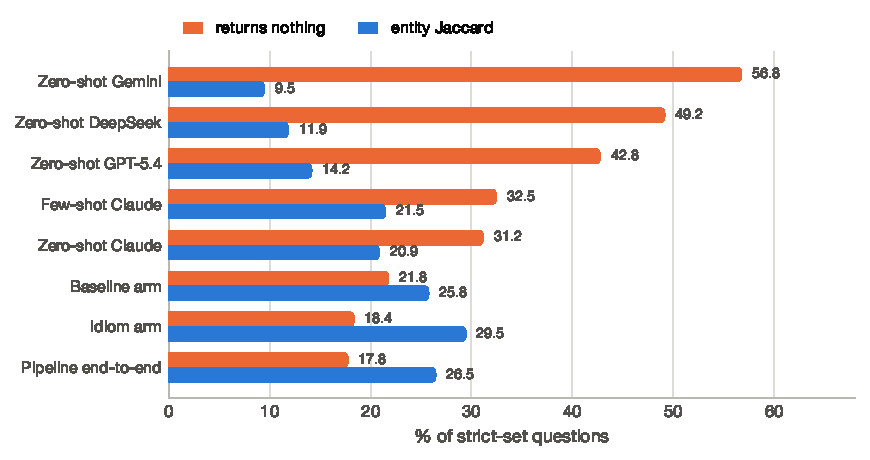
\includegraphics[width=0.8\textwidth]{figures/fig_empty_rate.pdf}
  \caption{How often each system returns nothing, against its accuracy.}
  \label{fig:empty}
  \tabnote{Every gold query on the strict set returns at least one row, so an empty result is always wrong.}
\end{figure}

\begin{figure}[H]
  \centering
  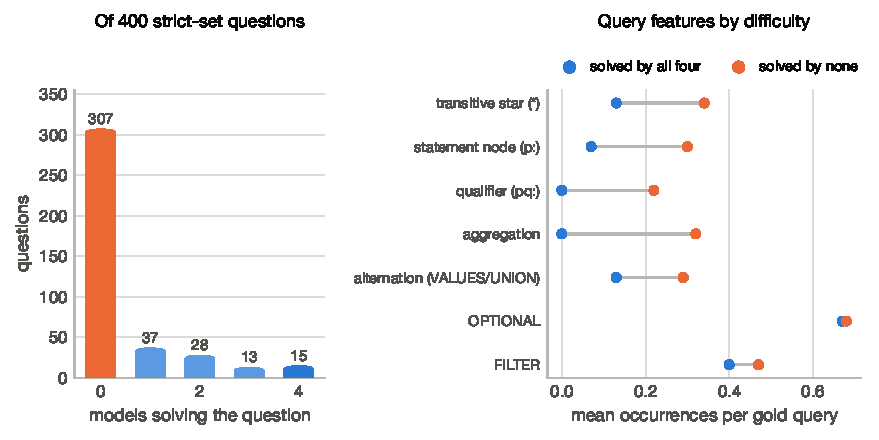
\includegraphics[width=0.8\textwidth]{figures/fig_cross_model_agreement.pdf}
  \caption{Cross-model agreement and what distinguishes the hard questions.}
  \label{fig:crossmodel}
  \tabnote{Left: how many of the four zero-shot models solve each question. Right: mean occurrences of each construct per gold query, comparing questions no model solved with those all four solved. Qualifier access and aggregation appear at exactly zero in every question all four solved.}
\end{figure}

\begin{figure}[H]
  \centering
  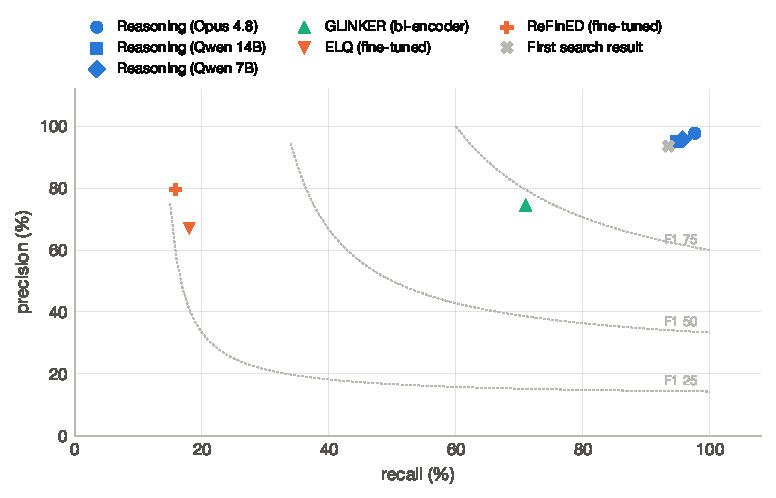
\includegraphics[width=0.8\textwidth]{figures/fig_linker_pr.pdf}
  \caption{The precision--recall signature of each linking paradigm.}
  \label{fig:linker-pr}
  \tabnote{Working split. Mention-level precision against recall for each linker.}
\end{figure}

\begin{figure}[H]
  \centering
  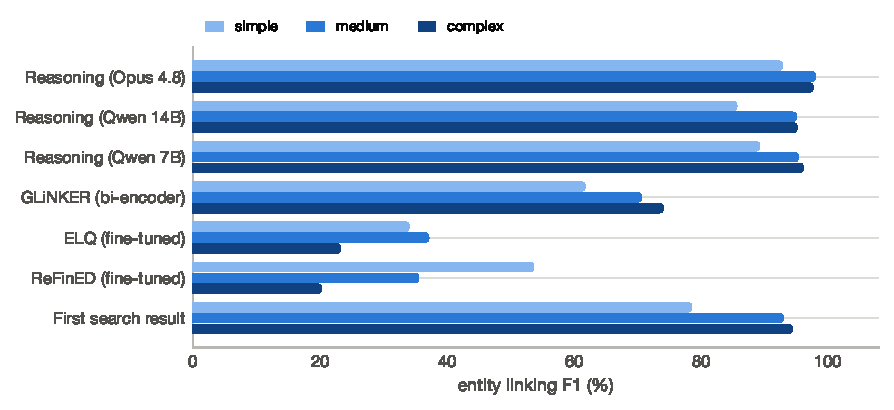
\includegraphics[width=0.8\textwidth]{figures/fig_linker_complexity.pdf}
  \caption{Linking F1 by query complexity.}
  \label{fig:linker-cx}
  \tabnote{Working split. Entity-linking F1 for simple, medium and complex queries.}
\end{figure}

\begin{figure}[H]
  \centering
  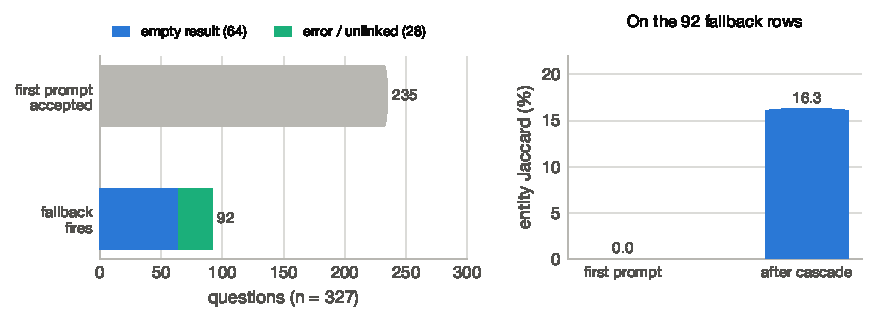
\includegraphics[width=0.8\textwidth]{figures/fig_cascade_fallback.pdf}
  \caption{Where the cascade's fallback fires, and what it recovers.}
  \label{fig:fallback}
  \tabnote{The fallback triggers on 28\,\% of questions, most often because the preferred query returned nothing. On exactly those rows the first prompt scores zero by construction.}
\end{figure}

\begin{figure}[H]
  \centering
  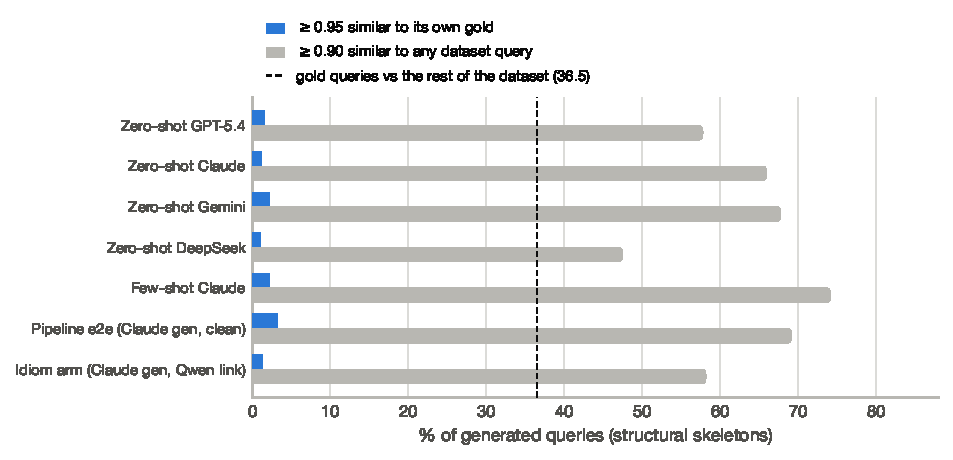
\includegraphics[width=0.8\textwidth]{figures/fig_memorisation.pdf}
  \caption{Structural similarity of generated queries to the benchmark.}
  \label{fig:memorisation}
  \tabnote{Skeletons compare query shape only.}
\end{figure}

\begin{figure}[H]
  \centering
  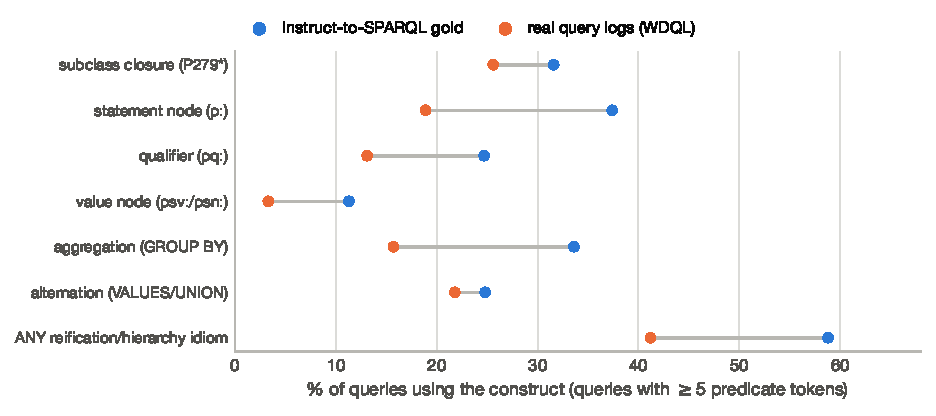
\includegraphics[width=0.8\textwidth]{figures/fig_wdql_bysize.pdf}
  \caption{Construct prevalence at matched query size.}
  \label{fig:wdql-size}
  \tabnote{Restricted to queries with at least five predicate tokens.}
\end{figure}

\begin{figure}[H]
  \centering
  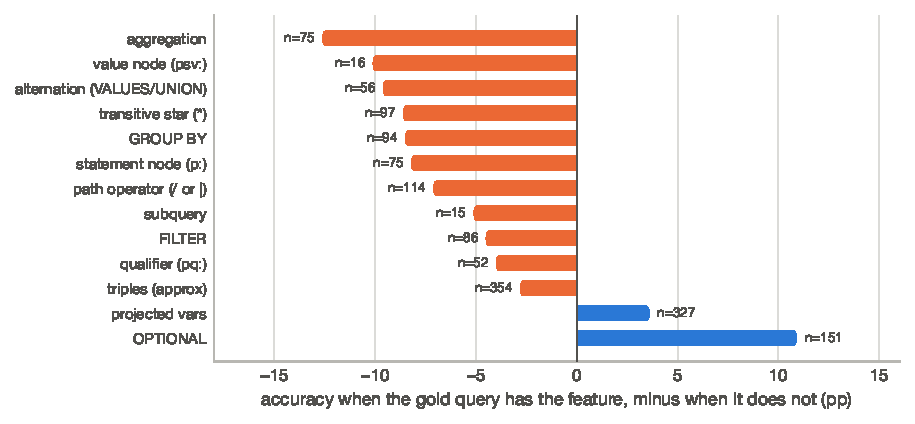
\includegraphics[width=0.8\textwidth]{figures/fig_structural_predictors.pdf}
  \caption{Gold-query features against achieved accuracy.}
  \label{fig:predictors}
  \tabnote{Group-mean differences, not predictive relationships: correlations are weak throughout ($|\rho| \leq 0.15$) and several features are rare. \textsc{optional} is the only feature associated with higher accuracy.}
\end{figure}
